\section{Background and Process}
\label{background}
\subsection{Project Scope}
\label{scope}
The team chose the project “AI4Agile: Developing AI-enabled tool support for user story refinement in JIRA” from SCORE 2021's project list to participate in the competition. The project is sponsored by Dr. Hoa Khanh Dam from Univeristy of Wollongong in Australia. It stemmed from Dr. Dam's research in the intersection of Software Engineering and Artificial Intelligence \cite{dam1,dam2,dam3}. 

The project proposed four primary requirements \cite{proposal}:

\begin{enumerate}
	\item Recommend user stories that are decomposed from an epic.
	\item Recommend smaller user stories to be split from bigger user stories.
	\item Recommend subtasks derived from a user story.
	\item A visualization (e.g. a graph) of epics, user stories and tasks, and their relationships.
\end{enumerate}

In addition, the application must be integrated and easily deployed into the platform of Atlassian’s Jira software, a widely used software project management tool that provides a marketplace for add-on applications \cite{jira1}. 

\subsection{Teams and Stakeholders}
We entered the SCORE competition upon recommendation by our faculty advisor Dr. Bolong Zeng. The four team members who participate in the competition are all senior students in the Software Engineering major at Washington State University, Everett, USA. We complete the project as part of our Software Requirement and Senior Design Capstone courses. \footnote{As part of this year's theme of our Senior Design Capstone projects (Avatar: the Last Airbender), the team is named Team Katara.} 

Among the list of projects, the team chose AI4Agile since the team were interested in working with AI for the first time. The idea of intersecting AI with Software Engineering (SE) was also intriguing, particular for four Software Engineering major students. The project is essentially a meta-project on SE as we would be developing an SE tool that helps with the SE process, while conducting our own SE process. 

The team enlisted the help of several faculty and industry mentors/advisors. Dr. Zeng is the faculty advisor who supervises the team's process and review our work products. As the team has no prior experience with AI and Natural Language Processing (NLP), we ask for advice from Prof. Jeremy Thompson, whose main expertise is in these fields. We also contacted Dr. Dam, the SCORE sponsor as soon as the team started our work. Dr. Dam provided us with his previous research and publications, from which AI4Agile was born, as well as sample data that he used in the past. 

As the project is a tool for software developers, we were fortunate enough to have a senior project manager, Skip Baccus, from Microsoft who agreed to fulfill the role as a domain expert. Throughout the project, he works with us as both a mentor and a stand-in for potential client. All people mentioned above rounded up the stakeholders in the project. Team member Aric Monary served as a team liaison to coordinate communications among all involved parties.

\subsection{Team Process}
The team adopted the agile process for the project. The team met a minimum of 2 times per week to go over documentation and the implementation work on the project. These meetings led into the scrum meeting with our business mentor every Tuesday. Each time a new component was implemented, we debrief the mentor during the scrum to solicit feedback from his perspective. In between these meetings, the team worked on their own assigned tasks, while the faculty advisor reviewed our documentations. Figure \ref{fig:acd} shows the major activities of the team on a weekly basis. 

\begin{figure}
\centering
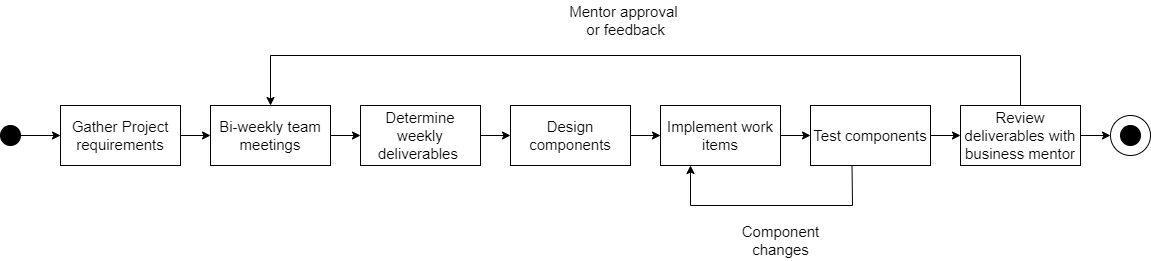
\includegraphics[width=\textwidth,keepaspectratio]{./figure/ActivityDiagram.png}
\caption{Activity Diagram outlining the SE processes}
\label{fig:acd}
\end{figure}

The team started by studying on Dr. Dam's paper, mainly \cite{dam1}, and brainstorming concepts that we think are important to the project. The team then split into doing research on various key issues, such as Jira API, NLP, etc. based on individual strengths and interests. Meanwhile, the entire team participated in regular requirement solicitation with the mentor to refine the intial scope in the project proposal. Throughout the process we obtain key understanding on agile process itself, and how the tool can best assist within the project scope. The requirements are presented in more details in Section \ref{requirement}. As we were finalizing major features to implement, the team simultaneously started early coding to experiment with implementation based on our earlier research. 

The development effort mainly consists of two parts: AI and UI components.  The AI components were of high priority through majority of the project. Three members each focused on one of the three primary requirements needed for the AI, while the fourth member focused on building UI for the visualization tool. As the project came to a close, we moved the UI portion as top priority while AI development was completed. As our final milestone, we demonstrated the functional prototype of the tool to our stakeholders by conducting walkthroughs of major use cases. Figure \ref{fig:timeline} presents the project timeline, with key work tasks and dates noted. Figure \ref{fig:responsibility} provides an overview of responsibility assignments for functionalities of the add-on.

\begin{figure}
\centering
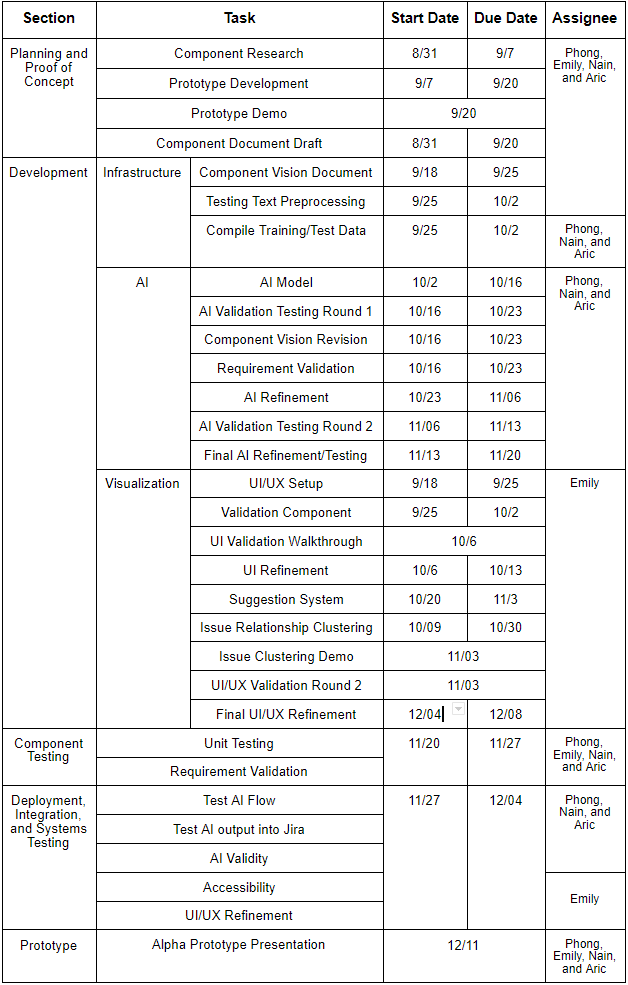
\includegraphics[width=\textwidth,keepaspectratio]{./figure/ProjectTimeline.png}
\caption{Project Timeline}
\label{fig:timeline}
\end{figure}

\begin{figure}
\centering
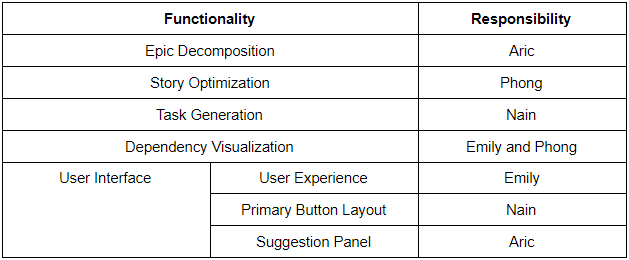
\includegraphics[width=\textwidth,keepaspectratio]{./figure/FunctionResponsibility.png}
\caption{Function Responsibility Breakdown}
\label{fig:responsibility}
\end{figure}